%%
%% This is file `sample-acmtog.tex',
%% generated with the docstrip utility.
%%
%% The original source files were:
%%
%% samples.dtx  (with options: `acmtog')
%% 
%% IMPORTANT NOTICE:
%% 
%% For the copyright see the source file.
%% 
%% Any modified versions of this file must be renamed
%% with new filenames distinct from sample-acmtog.tex.
%% 
%% For distribution of the original source see the terms
%% for copying and modification in the file samples.dtx.
%% 
%% This generated file may be distributed as long as the
%% original source files, as listed above, are part of the
%% same distribution. (The sources need not necessarily be
%% in the same archive or directory.)
%%
%% The first command in your LaTeX source must be the \documentclass command.
\documentclass[manuscript,review,anonymous]{acmart}

%% NOTE that a single column version is required for 
%% submission and peer review. This can be done by changing
%% the \doucmentclass[...]{acmart} in this template to 
%% \documentclass[manuscript,screen]{acmart}
%% 
%% To ensure 100% compatibility, please check the white list of
%% approved LaTeX packages to be used with the Master Article Template at
%% https://www.acm.org/publications/taps/whitelist-of-latex-packages 
%% before creating your document. The white list page provides 
%% information on how to submit additional LaTeX packages for 
%% review and adoption.
%% Fonts used in the template cannot be substituted; margin 
%% adjustments are not allowed.

\usepackage{amsmath} 
\usepackage{subfig}
\usepackage{booktabs}
\usepackage{multirow}
\usepackage[ruled,vlined]{algorithm2e}
\usepackage{bbm}

%%
%% \BibTeX command to typeset BibTeX logo in the docs
\AtBeginDocument{%
  \providecommand\BibTeX{{%
    \normalfont B\kern-0.5em{\scshape i\kern-0.25em b}\kern-0.8em\TeX}}}

%% Rights management information.  This information is sent to you
%% when you complete the rights form.  These commands have SAMPLE
%% values in them; it is your responsibility as an author to replace
%% the commands and values with those provided to you when you
%% complete the rights form.
\setcopyright{acmcopyright}
\copyrightyear{2021}
\acmYear{2021}
\acmDOI{10.1145/1122445.1122456}

%%
%% These commands are for a JOURNAL article.
%\acmJournal{TOG}
%\acmVolume{37}
%\acmNumber{4}
%\acmArticle{111}
%\acmMonth{8}

%%
%% Submission ID.
%% Use this when submitting an article to a sponsored event. You'll
%% receive a unique submission ID from the organizers
%% of the event, and this ID should be used as the parameter to this command.
%%\acmSubmissionID{123-A56-BU3}

%%
%% The majority of ACM publications use numbered citations and
%% references.  The command \citestyle{authoryear} switches to the
%% "author year" style.
%%
%% If you are preparing content for an event
%% sponsored by ACM SIGGRAPH, you must use the "author year" style of
%% citations and references.
\citestyle{acmauthoryear}

\newcommand{\el}[1]{
        \textcolor{magenta}{EL: #1}}

\newcommand{\dk}[1]{
        \textcolor{blue}{DK: #1}}
        
\newcommand{\pmu}[1]{
        \textcolor{orange}{PM: #1}}

\DeclareMathOperator*{\argmin}{arg\,min}
%%
%% end of the preamble, start of the body of the document source.
\begin{document}

%%
%% The "title" command has an optional parameter,
%% allowing the author to define a "short title" to be used in page headers.
%\title{\dk{Sharing is Caring: Neighborhood Reuse for Privacy-Aware Collaborative Filtering Recommender Systems}}
\title{ReuseKNN: Neighborhood Reuse for Privacy-Aware Collaborative Filtering}

%Controlling for Data Diffusion in Collaborative Filtering Recommender Systems
%%
%% The "author" command and its associated commands are used to define
%% the authors and their affiliations.
%% Of note is the shared affiliation of the first two authors, and the
%% "authornote" and "authornotemark" commands
%% used to denote shared contribution to the research.
%\author{Anonymous}
% \author{Peter Müllner}
% \email{pmuellner@know-center.at}
% \affiliation{%
%   \institution{Know-Center Gmbh}
%   \city{Graz}
%   \country{Austria}
% }

% \author{Elisabeth Lex}
% \affiliation{%
%   \institution{Graz University of Technology}
%   \city{Graz}
%   \country{Austria}}
% \email{elisabeth.lex@tugraz.at}

% \author{Dominik Kowald}
% \email{dkowald@know-center.at}
% \affiliation{%
%   \institution{Know-Center Gmbh}
%   \city{Graz}
%   \country{Austria}
% }

%%
%% By default, the full list of authors will be used in the page
%% headers. Often, this list is too long, and will overlap
%% other information printed in the page headers. This command allows
%% the author to define a more concise list
%% of authors' names for this purpose.
%\renewcommand{\shortauthors}{Trovato and Tobin, et al.}

%%
%% The abstract is a short summary of the work to be presented in the
%% article.
\begin{abstract}
todo
\end{abstract}

%%
%% The code below is generated by the tool at http://dl.acm.org/ccs.cfm.
%% Please copy and paste the code instead of the example below.
%%

%%
%% Keywords. The author(s) should pick words that accurately describe
%% the work being presented. Separate the keywords with commas.
\keywords{Todo; TODO}


%%
%% This command processes the author and affiliation and title
%% information and builds the first part of the formatted document.
\maketitle

\section{Introduction}
\pmu{RQ1: Utility-privacy trade-off. Outdegree vs. MAE + size of mentorset}
\pmu{RQ2: Debiasing. skewness plots}


\begin{figure*}[!htb]
    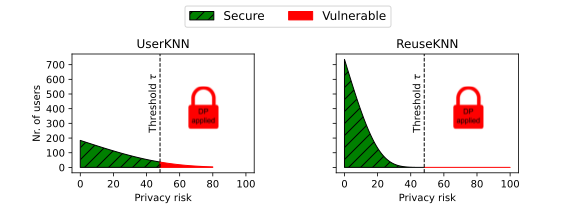
\includegraphics[width=\textwidth]{figures/intro.pdf}
    \caption{In traditional UserKNN the rating data of Bob, Tim, and John are utilized for generating recommendations for target user Alice. Alice's knowledge is restricted to her data, the algorithm used, and the recommendations. By adding specific ratings and querying recommendations, Alice could infer the user profiles of Bob, Tim, and John.
    We propose a novel family of methods, i.e., ReuseKNN, in which Alice reuses the same set of neighbors for all queries. Here, all queries are redistributed to Bob. As such, inference on Tim and John is impossible, for the price of an increased chance of successful inference on Bob.}
\end{figure*}

\pmu{zero-sum game regarding inference risk, we do not reduce total inference risk, we just redistribute it to a small set of mentors}

\pmu{Intro problems: too much related work? attacks on statistical databases not in focus (de-anonymization), clear contributions, knowledge of the target user}

\el{you should have this structure for the intro in mind: 1-2 introductory sentences, problem, scope and objective, approach, contributions and findings}

\el{You can start more briefly, so shorten the first paragraph a bit - CF is a frequently used recsys technique. However, CF recommender systems can have privacy issues since recommendations are produced based on data that is collected from the $k$-nearest neigbors of a target user. --> that will make the intro part more concise and instantly highlight the problem.}
Modern recommender systems are often based on collaborative filtering. 
In this paradigm, users collaboratively share their knowledge to provide recommendations for a target user. Thus, the widsom of the crowd serves defines what the target user's recommendations consist of.
In this regard, paying close attention to not leaking any private user information is a necessity requested by users~\pmu{cite} and to be guaranteed by state-of-the-art recommender systems.

\el{Now, you need to say early on what this work is about. In this work, In our work, we aim to increase the privacy of users within the community by proposing modifications to the architecture of $k$-nearest neighbors recommendation methods.}
\el{A rich body of research exists on preserving users' privacy in recommender systems that can be categorized into four strands - here, I would point to the respective recsys handbook chapter for an overview}: To provide users with their required privacy needs when participating in a recommender system, four strands of research evolved \el{if you say "four strands", list them with either (i) or first, second}: data privacy, algorithmic privacy, user-defined privacy, and architectural privacy \pmu{use names in community} \el{add references here}. 
In data privacy, random noise is added to the data to obfuscate the true user profile.
A rich toolkit to guarantee some boundary on the data disclosure is given by differential privacy~\cite{dwork2014algorithmic}.
Algorithmic privacy aims to develop algorithms that do not expose the user to any threats on her privacy.
Furthermore, it is questionable, whether a recommender system's adherence to a user's sensitive data yields sufficient advantages when compared to the increased exposure of a user's data.
User-defined privacy enables a user with all means to control her data. 
In detail, she \el{use the gender unspecific "they" also for a single user} decides what data to share and what data to not share with the recommender system.
Often, privacy threats are not primarily posed by the algorithm or the data itself, but by the architecture of the recommender system. 
For example, federated learning is widely-used to generate recommendations in a distributed setting.
Here, no data ever leaves the device of a user.
Users only shares updates and thus, nonsensitive information, with the community.
However, research is aware that even in this case, private information could be inferred by a malicious user. 
In this regard, research in~\cite{ramakrishnan2001being} illustrated that especially users of diverse taste, i.e., straddlers, are susceptible to privacy threats, such as inference of rating data and de-anonymization attacks similar to attacks in statistical databases. \dk{we can link this here to more novel works regarding explainability and serendipity in recommender systems because this problem especially occurs when this is given}

In our work, we focus on increasing the privacy of users within the community by proposing modifications to the architecture of $k$-nearest neighbors recommendation methods.
The threat of disclosing private data lies in the neighboring users' ''mentoring" of the target user, i.e., ''student", by providing their data to the recommender system in order to generate recommendations.
For example, assume that Alice rated James Bond and queries a new movie to be recommended by the recommender system, which responds with Star Wars.
In $k$-nearest neighbors, the recommendations are based on the most similar neighbors to the target user.
Assume that $k=1$ and thus, Bob is the only neighbor of Alice.
Then, Bob is only in the neighborhood of the target user Alice, if Bob shares at least one rating with Alice.
Since Alice rated James Bond, it can be inferred that Bob rated James Bond.
As the recommendation presented by the recommender system is Star Wars, Bob must have rated both, i.e., James Bond and Star Wars.

Typically, the number of neighbors lies in the range of $[30, 50]$~\pmu{cite}.
Furthermore, a user's profile comprises many ratings.
Here, inference is not as simple as in our example with a single neighbor, but still feasible.
Given all users rated more than one movie, and the number of neighbors $k>1$, then Alice can neither identify a user, nor infer ratings.
The presence of multiple candidates protects the anonymity of each user, i.e., $k$-anonymity.
However, Alice could generate fake users similar to her, fix James Bond and alter the remaining ratings.
If most variations do not yield the same recommendation, i.e., Star Wars, Alice's confidence that her neighbors rated James Bond may increase.
The more often Bob is in the neighborhood of Alice, the higher the chances of successful inference through Alice.
How often Bob is in the neighborhood of other users, is therefore correlated to Bob's risk of disclosure.
Thus, in the work at hand, privacy risk is defined as the number of times, a user mentors a target user.



Our work aims to reduce the number of queries per mentor, so that inference and de-anonymization attacks are not feasible. 
For example, Alice queries ten recommendations, which are each based on a single mentor.
Thus, each mentor is queried once, which poses privacy threats of Alice towards her mentors.
In our work, we reduce the number of queries per mentor by reusing the mentors of the first query for the succeeding queries.
In this setting, we modify Alice's neighborhood such that her ten queries no longer aim at ten mentors, but at only one.
Therefore, we protected nine users by transferring the privacy risk towards the tenth user.
However, we illustrate that also this single highly-susceptible user can be protected.
In this study at hand, we simulate this user by creating a fake user, with a similar, but not identical, user profile.
Through this simulation, also the real user can be protected and the privacy risk is transferred to our fake user. \dk{cool, wie machen wir das genau?}




\pmu{attacks on statistical databases necessary? what's the benefit?} \dk{nein, so wie es ist, ist es gut, also nur einmal erwähnt beim citen des papers, dann wuered ich wie oben erwaehnt noch sagen, dass explainability und serendipity die Gefahr noch erhoehen und hier ein paar neue Papers zitieren}

\begin{figure*}[!htb]
    \centering
    \includegraphics[width=\textwidth]{figures/approach.pdf}
    \caption{Here, the detailed impact of our approach, is illustrated with a basic example. Here, $Q_1, Q_2$ and $Q_3$ are Alice's queries and Mentors refers to Alice's utilized mentors. In UserKNN, target user Alice's recommendations are based on the rating data of Bob, Tim, and John. Thus, we call Bob, Tim, and John mentors of target user Alice. 
    Since each mentor rated at least one item she has rated, Alice knows that all mentors rated James Bond. Plus, upon recommendation of, e.g., Cast Away, she knows that some of her mentors also rated Cast Away. By probing, i.e., gradually adding specific ratings and querying recommendations, Alice could infer the user profiles of Bob and John.
    Our proposed family of methods, i.e., ReuseKNN, redistributes all queries to Bob. Thus, arget user Alice cannot infer Tim's and John's rating data, whereas the chance of successful inference of Bob's rating data increases. Moreover, since Alice's recommendations are solely based on Bob, she could infer all of Bob's data with only three queries, which lead to three recommendations leaking Bob's rating data.
    }
    \label{fig:approach}
\end{figure*}

\pmu{ It is important to note that if multiple mentors contribute to Alice's recommendations, the relative contribution of a single mentor decreases, as can be observed in Equation~\ref{eq:knn}.
Therefore, it becomes harder for Alice to conduct an inference attack on a single mentor.
One may be tempted to conclude that utilizing more mentors leads to the mentors being strongly protected against inference. 
However, we note that Alice could easily bypass this protection by extensive probing and querying recommendations~\cite{calandrino2011you}.
Furthermore, the recommender could utilize fewer neighbors to generate recommendations.
As such, not as many users would be mentors of the target user and thus, the average number of users a target user could perform inference on, would decrease.
However, decreasing the number of neighbors, i.e., mentors, would substantially decrease the quality of the generated recommendations~\cite{herlocker1999algorithmic,herlocker2002empirical}}

\section{Approach}
Traditional $k$-nearest neighbors collaborative filtering recommender system generates an estimated rating score for user $u$ and item $i$.
In our work, all those users that rated $i$ are called \emph{neighbors} of a \emph{target user} for item $i$.
Typically, the recommender system selects $k$ neighbors based on which its estimation of the target user's rating score of item $i$ is based on.
Thus, these $k$ selected neighbors, i.e., $N^k_{u, i}$, contribute to target user $u$'s recommendations.
In our work, we call all those users that contributed to at least one of target user $u$'s recommendations \emph{mentors} of $u$.
More formally, the set of mentors of $u$ is $M_u = \bigcup_{i \in Q_u} N_{u, i}$, where $Q_u$ is the set of items, for which $u$ queries an estimated rating score.
% In our toy example of ReuseKNN in Figure~\ref{fig:approach}, Alice is the target user $u$ querying recommendations.
% For recommending item $i$, i.e., Titanic, Bob, Tim, and John are neighbors $N_{u, i}$, as they rated Titanic and could serve as basis for estimating Alice's rating for Titanic.
% However, out of all three neighbors, only Bob is selected to be a mentor (i.e., Bob $ \in M_{u, i}$) for Alice querying Titanic. 
% Thus, the estimation of the rating score of Alice for Titanic is solely based on Bob.

Despite $u$ is only aware of her own data, the algorithm, and the recommendations she receives, $u$ could infer the rating data of her neighbors~\cite{calandrino2011you,ramakrishnan2001being}.
As such, all mentors of $u$ are susceptible to $u$'s inference attacks.
Moreover, the paper at hand focuses on a centralized implementation of UserKNN.
With this, the recommender system is responsible for generating the estimated rating score $\hat{r}_{u, i}$ and users (e.g., a target user and its neighbors) only communicate with the recommender system itself.
As such, the recommender system must be equipped with privacy-preserving methods to (i) compute the similarity between two users and (ii) maintain a dictionary, indicating what user rated which items.
Recent research proposes a plethora of privacy-preserving methods to realize the above points.
For this reason, we leave this points open and concentrate on how a recommender system shall select a target user's neighbors in order to decrease the possibility of inference.

\subsection{UserKNN}
\label{subsec:userknn}
In collaborative recommender systems, users' recommendations are based on collaboration among users and as such, exploitation of other users' data.
In the case of UserKNN, the recommender system generates an estimation $\hat{r}_{u, i}$ of a target user $u$'s preference for item $i$ by leveraging the data of $u$'s top $k$ neighbors $N^k_{u, i}$ for item $i$ according to some similarity measurement $sim$, in detail
\begin{equation}\label{eq:knn}
    \hat{r}_{u, i} = \frac{\sum_{n \in N^k_{u, i}} sim(u, n) \cdot r_{n, i}}{\sum_{n \in N^k_{u, i}} sim(u, n)}
\end{equation}
where $r_{n, i}$ is the rating of neighbor $n$ for item $i$ and $sim$ denotes a similarity function which measures the conformity between target user $u$ and neighbor $n$.
Typically, cosine-similarity is used as a similarity function, as it usually results in a better recommendation accuracy than other similarity functions~\cite{bagchi2015performance}.
Furthermore, we pinpoint the observation that since $n$ is within the top $k$ neighbors of user $u$ and item $i$, $n$ is also a mentor of $u$ and belongs to the set of $u$'s mentors $M_u$.

In our toy example as given in Figure~\ref{fig:approach}, Alice is the target user querying recommendations from the recommender system, i.e., UserKNN.
For Alice's first query, i.e., Star Wars, UserKNN selects Bob to be a neighbor of Alice, since Bob is the only user that rated both, James Bond and Star Wars.
For Alice's second query, i.e., Cast Away, UserKNN selects Bob and John to be neighbors of Alice.
Thus, the set of neighbors that contributed at least once to Alice's recommendations, i.e., Alice's mentors, now comprises Bob and John.
Finally, in a query for Titanic, UserKNN, selects Bob, Tim, and John as neighbors for Alice.
In total, UserKNN has selected three users, i.e., Bob, Tim, and John to be neighbors of target user Alice.
Thereby, Bob, Tim, and John contribute to at least one of Alice's recommendations.
As such, Bob, Tim, and John are mentors of Alice.
Hence, there is the possibility that Alice could infer the rating data of Bob, Tim, and John.
%For example, upon recommendation of Cast Away, Alice knows that some of her mentors rated Cast Away.
%By adding ratings and querying recommendations, she could infer the rating data of Bob and John.
% It is important to note that if multiple mentors contribute to Alice's recommendations, the relative contribution of a single mentor decreases, as can be observed in Equation~\ref{eq:knn}.
% Therefore, it becomes harder for Alice to conduct an inference attack on a single mentor.
% One may be tempted to conclude that utilizing more mentors leads to the mentors being strongly protected against inference.
% However, we note that Alice could easily bypass this protection by extensive probing and querying recommendations. \pmu{add reference or choose other argument}

\subsection{Threat Model}
In traditional $k$-nearest neighbor algorithms, the estimated rating score $\hat{r}_{u, i}$ of target user $u$ for a item $i$ depends on the top k neighbors $N^k_{u, i}$ selected by the recommender system.
For a succeeding item $j$, the estimated rating score $\hat{r}_{u, j}$ then depends on other top k neighbors $N^k_{u, j}$.
As our example in Figure~\ref{fig:approach} shows, after recommending Star Wars, Cast Away, and Titanic, target user Alice's set of mentors comprises Bob, Tim, and John.
Bob and John contribute to three respectively two recommendations and Tim contributes to one recommendation. 
Consider Alice adding a rating for Titanic to her existing rating for James Bond.
If the recommender system yields the recommendation Star Wars, Alice could infer that Bob rated Star Wars. 
This by itself poses a severe breach of Bob's privacy.
Plus, even incomplete knowledge of Bob's rating data is a strong threat to Bob's privacy.
For example, this incomplete knowledge could boost the effectiveness of other kinds of attacks, e.g., Sybil attacks~\cite{calandrino2011you}.
Furthermore, since the number of recommendations in which Bob's contributes to is higher than for Tim, Bob is more prone to inference attacks than Tim, since Bob reveals more about his rating data~\cite{ramakrishnan2001being}.
However, technically, Alice could still infer not only the rating data of Bob, but also of John, and Tim.

From a privacy perspective, a user could attain two roles: \emph{susceptible} and \emph{attacker}.
If the recommender system selects user $n$ to serve as neighbor in at least one recommendation for target user $u$, $n$ is also a mentor of $u$.
Due to $n$ being $u$'s mentor, $n$ attains the role of a susceptible.
That means that $n$ is susceptible to $u$'s inference attacks.
Clearly, $u$ then attains the role of an attacker.
Also, we highlight that in typical $k$-nearest neighbor collaborative filtering recommender system, a user (i) queries recommendations and (ii) contributes in the recommendations for other users.
As such, a user could be susceptible to inference, but still be an attacker to other users.

\subsection{ReuseKNN}
\label{subsec:reuseknn}
In order to provide high quality recommendations for one user whilst ensuring privacy of others, the paper at hand proposes a novel family of neighborhood selection methods, i.e., ReuseKNN.
Instead of utilizing fewer neighbors per recommendation and as such, decreasing the number of mentors per target user, ReuseKNN decreases the number of mentors per target user whilst not limiting the number of neighbors that contribute to a recommendation
As such, it equips the users with increased privacy and provides them high quality recommendations.
In particular, the key feature of ReuseKNN is to reuse a target user's previously utilized neighbors whenever feasible.
With that, it reduces the number of users that are added to the target user's set of mentors with every recommendation.
For example, as can be seen in Figure~\ref{fig:approach}, ReuseKNN redirects queries for multiple neighbors, i.e., Bob, Tim, and John, to Bob.
Thus, all recommendations for Alice are based on only Bob who serves as mentor, whereas Tim and John are protected against inference.
More detailed, for Alices first recommendation, i.e., Star Wars, ReuseKNN is inline with UserKNN (cf. Section~\ref{subsec:userknn}) and selects Bob as neighbor.
However, in the second recommendation, i.e., Cast Away, ReuseKNN differs from UserKNN.
Instead of increasing Alice's set of mentors by using Tim or John as neighbors, ReuseKNN reuses the mentors already available to Alice.
In detail, since mentor Bob already rated Cast Away, ReuseKNN reuses Bob as neighbor in Alice's recommendation of Cast Away.
Similarly, in the third recommendation, i.e., Titanic, ReuseKNN does not add any additional mentors to Alice's set of mentors, since mentor Bob rated Titanic.
Overall, instead of selecting all three users as mentors as UserKNN did, and thus exposing all users' data to Alice, ReuseKNN reuses Alice's mentors as neighbors in her recommendations and thereby, prohibits inference attacks by Alice on the other users not used as mentors.
Specifically, ReuseKNN employs our family of neighborhood-selection methods that restrict the number of distinct mentors per target user.
For $Q_u$ being the set of items for which a target user $u$ queries estimated rating scores and $N^k_{u, i}$ being the top $k$ neighbors of $u$ for item $i$ used in estimating the rating score of $i$, ReuseKNN aims to identify the smallest set of distinct neighbors such that it minimizes the cardinality of $M_u = \cup_{i \in Q_u} N^k_{u, i}$
whilst keeping the quality of $u$'s recommendations high.

Traditionally, cosine-similarity is utilized to identify neighbors.
In detail, neighbors are selected based on their similarity to the target user and thus, shall improve utility, i.e., accuracy of the target user's recommendations.
Our family of methods does not only consider the similarity $sim(u, n)$ between target user $u$ and neighbor $n$, but also the extent $reusability(n|u)$ to which the recommender system could reuse $n$'s rating data in $u$'s future recommendations.
We formalize this trade-off between utility and privacy as weighted average between similarity and reusability.
\begin{equation}
    \label{eq:tradeoff}
    score(n|u) = \lambda \cdot rank(sim(u, n)) + (1 - \lambda) \cdot rank(reusability(n|u))
\end{equation}
, where the recommender system, i.e., ReuseKNN, selects the highest scored $k$ neighbors $n$ to contribute to target user $u$'s recommendations and thus, serve as mentors for $u$.
Furthermore, $\lambda \in [0; 1]$ is used to trade utility (i.e., $sim$) for privacy (i.e., $reusability$).
Moreover, we do not directly utilize the similarity and reusability scores, since those two measurements cannot be compared as they have different scales depending on the dataset used.
Instead, we make use of a ranking of these two scores, in order to propose a general approach, applicably to any dataset.
By focusing on selecting neighbors that are reusable, ReuseKNN reuses neighbors from previous recommendations and as such, keeps the set of mentors of $u$ small.
Hence, most users are not utilized as mentors and thus, are strongly protected against inference attacks by a target user.
In the following sections, we describe our family of neighborhood-selection strategies utilized in ReuseKNN.

\subsubsection{Implicit Neighborhood Reuse}
\label{subsubsec:implicitreuse}
In this work, we propose to reuse mentors of a target user in future recommendations, such that the average susceptibility to inference attacks is alleviated, whilst preserving the quality of recommendations, the target user receives.
We rely on neighborhood-selection methods to identify a set of mentors, which are reusable as neighbors in future recommendations.
Our implicit neighborhood reuse method do not explicitly reuse neighbors, but create an artificial bias towards selecting those users in all future recommendations.
Neighbors are selected not only based on similarity, but based on a trade-off between similarity and reusability as outlined in Equation~\ref{eq:tradeoff}.
In detail, our implicit neighborhood reuse schema is illustrated in Algorithm~\ref{algo:implicit_neighborhood}.
In the following paragraphs, we discuss two methods, i.e., \emph{Popularity} and \emph{Gain}, which increase the reusability of mentors selected by the recommender systems.

\begin{algorithm}[!htb]
    \SetAlgoLined
    \DontPrintSemicolon
    \SetKwInOut{Input}{Input}
    \Input{Target user $u$ that queries estimated rating for item $i$, neighbors  $N_{u, i}$, and number of neighbors $k$ used in a recommendation.}
    \KwResult{Set $N^k_{u, i}$ of top $k$ neighbors used for computing the estimated rating score (cf. Equation~\ref{eq:knn}).}
    Rank all $n \in N_{u, i}$ according to $score(n|u)$ \tcp*{High $score(n|u)$ means high rank}
    $N^k_{u, i}$ = $\{k$ top ranked neighbors$\}$ \\
    \Return $N^k_{u, i}$
    \caption{Implicit Neighborhood Reuse Schema}
    \label{algo:implicit_neighborhood}
\end{algorithm}

\paragraph{Popularity}
Intuitively, the more popular an item, the more likely it is that a target user will query an estimated rating score for this item.
Our \emph{Popularity} method relies on this observation and thus, quantifies, for how many recommendations the recommender system could reuse the user's data.
That means, that it promotes neighbors, if they rated a lot of popular items.
Also, it penalizes neighbors that rated lots of unpopular, or only a few items.
In detail, the reusability score of neighbor $n$ is defined as
\begin{equation}
    reusability(n|u) = reusability(n) = \sum_{r_{n, i} \in R_n} \frac{|\{ v \in U: \exists r_{v, i} \in R_v \}|}{|U|}
\end{equation}
where $R_n$ are the ratings of user $n$ rated and $U$ is the set of all users.
Here, $reusability$ is the sum of the item popularities, neighbor $n$ rated.
As such, it measures the expected number of a random target user's recommendations, in which $n$ could contribute to.
Furthermore, we note that here, $reusability$ does not depend on target user $u$ and thus, it does only measure the $reusability$ of a neighbor with respect to the average user.

\paragraph{Gain}
When generating an estimated rating score for target user $u$, the recommender system utilizes the ratings $R_n$ of a neighbor $n$.
In general, the recommender system tries to select those neighbors for a target user, whose rating data could be reused for the target user's future recommendations.
That means that $R_n$ should cover most of the target user's future queries, i.e., $Q_u$.
Obviously, the recommender system does not know, for what items target user $u$ will query ratings in the future. 
Instead of asking how much of a student's future ratings a neighbor could cover, \emph{Gain} asks, how much of a target user's ratings a neighbor could have covered in the past, i.e., how much ratings the target user could have gained from neighbor $n$.
Thus, \emph{Gain} gives the fraction of a target user $u$'s rated items, for which neighbor $n$ could have provided her rating data, i.e., 
\begin{equation}
    reusability(n|u) = \frac{|I_u \cap I_n|}{|I_u|}
\end{equation}
where $I_u$ are the items rated by target user $u$ and $I_n$ are the items rated by neighbor $n$.
In contrast to \emph{Popularity}, we underline that \emph{Gain} is a personalized implicit neighborhood selection method, as it calculates the $reusability$ of a neighbor with respect to a specific target user.
Thus, a neighbor not reusable for one student could be highly reusable for another student.

\subsubsection{Explicit Neighborhood Reuse}
Contrary to the implicit neighborhood methods presented above, explicit neighborhood reuse methods do not only create an artificial bias for implicitly selecting reusable users as neighbors, but explicitly reuse as many neighbors as possible.
We highlight that \emph{UserKNN} and all implicit neighborhood reuse methods can be modified to reuse neighbors explicitly.
In detail, through combination with our explicit neighborhood reuse schema in Algorithm~\ref{algo:explicit_neighborhood}, we obtain our three explicit neighborhood reuse methods, i.e., \emph{UserKNN \& Reuse}, \emph{Popularity \& Reuse}, and \emph{Gain \& Reuse}.
Specifically, our explicit neighborhood reuse methods only select new neighbors and thus, add new neighbors to the set of mentors, if there are too less existing mentors that could be used for the target user's recommendation.
In other words, to increase others' privacy by not using those as mentors, our explicit neighborhood reuse methods force the recommender system to reuse a target user $u$'s mentors as neighbors in $u$'s recommendations whenever possible.
As such, they reuse mentors as neighbors even though there would be other neighbors with a higher similarity.
Eventually, to generate an estimated rating score, the $k$ most similar mentors are selected in order to foster utility.
In this regard, the explicit neighborhood reuse methods limit the incorporation of new mentors to a minimum, as such, they place a strong focus on privacy.

\begin{algorithm}[!htb]
    \SetAlgoLined
    \DontPrintSemicolon
    \SetKwInOut{Input}{Input}
    \Input{Target user $u$ that queries estimated rating for item $i$, mentors $M_{s}$ of $u$, neighbors $N_{u, i}$, and number of neighbors $k$ used in a recommendation.}
    \KwResult{Set $N^k_{s, i}$ of neighbors, used for computing the estimated rating score (cf. Equation~\ref{eq:knn}).}
    $M_{u, i}$ = $\{u$'s mentors that rated $i\}$ \\
    $n = \mathrm{max}\{k - M_{u, i}, 0\}$ \\
    \If{$n > 0$}{
        Rank all neighbors $n \in N_{u, i} \setminus M_{u, i}$ according to $score(n|u)$ \tcp*{High $score(n|u)$ means high rank}
        $M^{new}_{u}$ = $\{n$ highest ranked neighbors$\}$ \\
        $M_{u} = M_{u} \cup M^{new}_{u}$ \\
        $M_{u, i}$ = $\{u$'s mentors that rated $i\}$ \tcp*{Recompute set of $u$'s mentors that rated $i$}
    }
    $N^k_{u, i}$ = $\{$most similar $k$ mentors from $M_{u, i}\}$ \\
    \Return $N^k_{u, i}$
    \caption{Explicit Neighborhood Reuse Schema}
    \label{algo:explicit_neighborhood}
\end{algorithm}


\section{Experimental Setup}
\subsection{Evaluation Criteria}
\subsubsection{Privacy \& Utility}
As already mentioned above in Section~\ref{subsec:reuseknn}, the paper at hand proposes to reuse neighbors, in order to decrease the number of distinct neighbors, i.e., mentors per user.
With that, the mentors' privacy increases, since most mentors do not contribute to the recommendations to as many target users as otherwise.
From this perspective, decreasing the number of target users per mentor corresponds to mentors' decreased susceptibility to inference attacks conducted by malicious target users.
Therefore, we leverage a mentor $m$'s exposure as a measure for $m$'s privacy
Specifically, $m$'s exposure $\mathrm{Exposure}$ is the number of target users for which $m$ serves as mentor.
In detail, 
\begin{equation}
    \mathrm{Exposure}@k(m) = \sum_{s \in U} \mathbbm{1}_{M_s}(m)
\end{equation}
where $U$ is the set of all users and $\mathbbm{1}_{M_u}(m)$ is the indicator function of mentor $m$ being in the set of mentors $M_u$ for target user $u$.

Furthermore, to measure the quality of a target user's recommendations, i.e., utility, we rely on the widely-used Mean absolute error (MAE).
We prefer a rating-prediction based measurement, i.e., MAE, over top-$n$ recommendations based measurements, e.g., precision and recall, because the latter kind of measurements often utilize estimated rating scores to rank items.
As such, measuring the MAE allows a more general measurement of utility.
The MAE for a user $u$ is calculated by
\begin{equation}
    \mathrm{MAE}@k(u) = \frac{1}{|Q_u|} \sum_{i \in Q_u} |r_{u, i} - \mathcal{R}(u, i)| 
\end{equation}
where the recommender system $\mathcal{R}$ utilizes some neighborhood reuse method to select $k$ neighbors to estimate the rating scores for target user $u$'s queries $Q_u$.

\subsubsection{Redistribution of Inference Risk \& Fairness}
\pmu{if ratio remains at same level for growing k --> k has no effect on distribution privacy/utility tradeoff. if it increases skew of distribution --> privacy/utility tradeoff changes in an unequal way --> is that unfair?}
\pmu{skew increases -> dist more skewed to high ratios --> more users with low ratio --> option 1: smaller mae, option 2: larger nr of students, option 3: both. That means: some users stay at same level of privacy-utility, others get either better utility, or worse privacy, or both.}
\pmu{does our solution increase unfairness? unfairness is prevalent --> different ratios. if skew increases or decreases --> more unfairness}
\begin{equation}
    \mathrm{ratio}@k(u) = \frac{\mathrm{MAE}@k(u)}{\mathrm{Students}@k(u)}
\end{equation}

\pmu{$\mathrm{skew}(\mathrm{ratio}@k)$~\cite{kokoska2000crc}}

\subsubsection{Influence of Mentors}
\pmu{reliance on small set of mentors --> additional privacy threat? No!}

For two recommender system models, i.e., $\mathcal{P}$ and $\mathcal{F}$, the influence of mentor $m$ on the MAE is given by
\begin{equation}
    \mathrm{influence}@k(m) = \frac{1}{|U|}\sum_{u \in U} \big[ \mathrm{MAE}@k_{\mathcal{P}}(u) - \mathrm{MAE}@k_{\mathcal{F}}(u) \big]
\end{equation}
where $\mathcal{P}$ is the recommender system model trained on partial data, i.e. without $m$'s training data and $\mathcal{F}$ is the recommender system model trained on the full training set, i.e., with $m$'s training data.

\subsection{Datasets}
We conduct experiments on four different datasets, i.e., \emph{MovieLens 100k}\cite{harper2015movielens}, \emph{MovieLens 1M}~\cite{harper2015movielens}, \emph{Jester}~\cite{goldberg2001eigentaste}, and \emph{Goodreads}~\cite{DBLP:conf/recsys/WanM18,DBLP:conf/acl/WanMNM19}.

\begin{table}[!htb]
    \centering
    \begin{tabular}{l r r r r r r}
        \toprule
        Dataset & $|U|$ & $|I|$ & $|R|$ & Density & Avg. $|R| / |U|$ &  Avg. $|R| / |I|$ \\ \midrule
        MovieLens 100k & 943 & 1,682 & 100,000 & 6.3\% & 106.0 & 59.5 \\
        MovieLens 1M & 6,040 & 7,921 & 1,000,000 & 1.7\% & 165.6 & 269.9 \\
        Jester & 5,000 & 100 & 299,975 & 60.0\% & 59.9 & 2,999.8 \\
        Goodreads & 2,500 & 308,930 & 866,394 & 0.1\% & 346.6 & 2.8 \\ \bottomrule
    \end{tabular}
    \caption{Descriptive statistics of the four datased used in this study. $|U|$ is the number of users, $|I|$ is the number of items, $|R|$ is the number of ratings, Density denotes the density of the rating matrix, Avg. $|R| / |U|$ is the average number of ratings per user, and Avg. $|R| / |I|$ is the average number of ratings per item. Please note that we utilize a random sample of 5,000 users for Jester and a random sample of 2,500 users for Goodreads.}
\end{table}



\section{Results}
\dk{I guess, we have three patterns of results (i) the accuracy vs. outdegree/path length plots, (ii) the skewness plots, and (iii) the analysis of our re-used neighbors vs. the influential users based on the The Power of the Few paper}

\pmu{Our methods achieve better utility, why? Why is that no problem in regard to our following experiments?}
\pmu{First privacy measure. Whats the problem with that? refer to threat model.}
\pmu{Solution is the second measurement. What have we solved so far? --> path length with alpha (realistic setting)}
\pmu{skewness of ratio dist, refer to fairness, ... Good utility in exchange for good privacy?}
In Figure~\ref{fig:mae_vs_students}, the tradeoff between the MAE and the data leakage is illustrated for five different neighborhood-selection strategies.
As a baseline, we make use of standard $k$-nearest neighbors (KNN), in which a user $u$'s neighborhood is defined as the most similar users that have rated the item desired by $u$.
First, we observe that for all strategies, it is possible to decrease the number of students whilst preserving a low MAE.
However, it is noteworthy that our proposed strategies yield a far better privacy-utility tradeoff, since they assign a mentor to less students.
Most prominently, this behavior can be observed in settings, in which the MAE only slightly increases.
This is a clear advantage, since one does only have to trade a small amount of accuracy for a far better degree of privacy.
Employing a bias towards power-users and reusing neighbors yields the best results.
We note that the exhibited improvements of our strategies vanish with increasing MAE.
This may seem unintuitive at first sight.
However, large MAE scores typically occur when only a very few mentors (i.e., neighbors) contribute to a user's recommendation.
Thus, our proposed strategies are not able to advance the baseline given this small number of mentors.

\begin{figure}
    \centering
    \includegraphics[width=0.6\linewidth]{figures/ml-100k/k_vs_mae.png}
    \caption{Relationship between the mean absolute error and the number of neighbors $k$. Here, we compare traditional similarity-based neighborhood with our neighborhood strategies. We want to highlight that with our strategies, the behavior of UserKNN does not change whether neighbors are reused or not.}
    \label{fig:k_vs_mae}
\end{figure}

\begin{figure}[!htb]
    \centering
    \subfloat[t][]{\includegraphics[width=0.49\linewidth]{figures/ml-100k/outdegree_vs_mae.png}}
    \subfloat[t][]{\includegraphics[width=0.49\linewidth]{figures/ml-100k/skew_vs_k.png}}
    \caption{Experiments on the MovieLens 100k dataset. (a) Average outdegree of the sharing network plotted over the MAE for k=30 - 1 nearest neighbors built by our strategies with and without neighborhood reusage. 
    On average, our proposed neighborhood strategies yield a strongly increased level of privacy, whilst preserving utility. (b) Skewness of the ratio distribution, i.e., a user's mean absolute error divided by her number of students. Caused by the popularity biased dataset, the similarity-based neighborhood exhibits a peak for a small number of neighbors $k$. This behavior vanishes due smoothing by large $k$.
    In contrast, our proposed neighborhoods increase the right-skewness of the ratio distribution for increasing $k$.
    As we can assume the mean absolute error to stabilize for large $k$, we hypothesize that this skewness represents a substantial discrepancy in the number of students per user.}
\end{figure}

\begin{figure}[!htb]
    \centering
    \subfloat[t][]{\includegraphics[width=0.49\linewidth]{figures/ml-1m/outdegree_vs_mae.png}}
    \subfloat[t][]{\includegraphics[width=0.49\linewidth]{figures/ml-1m/skew_vs_k.png}}
    \caption{Experiments on the MovieLens 1M dataset. \pmu{strong popularity bias}}
\end{figure}

\begin{figure}[!htb]
    \centering
    \subfloat[t][]{\includegraphics[width=0.49\linewidth]{figures/jester/outdegree_vs_mae.png}}
    \subfloat[t][]{\includegraphics[width=0.49\linewidth]{figures/jester/skew_vs_k.png}}
    \caption{Experiments on the Jester dataset. \pmu{weak popularity bias}}
\end{figure}

\begin{figure}[!htb]
    \centering
    \subfloat[t][]{\includegraphics[width=0.49\linewidth]{figures/goodreads/outdegree_vs_mae.png}}
    \subfloat[t][]{\includegraphics[width=0.49\linewidth]{figures/goodreads/skew_vs_k.png}}
    \caption{Experiments on the Goodreads dataset. \pmu{extremely strong popularity bias, but no ratings}}
\end{figure}

\begin{table}[!htb]
    \centering
    \begin{tabular}{l r r}
        \toprule
        Method & Avg. Influence & Avg. Degree \\ \midrule
        UserKNN & 0.2541/0.2340 & 73.6000/81.7328 \\ 
        UserKNN + Reuse & 0.2360/0.2172 & 50.2000/47.4804 \\
        Popularity & 0.1778/0.1307 & 117.8000/42.7253 \\
        Popularity + Reuse & 0.1817/0.1387 & 14.7000/ 32.4115\\
        Gain & 0.1574/0.1338 & 60.6000/39.0498 \\
        Gain + Reuse & 0.1599/0.1414 & 56.2000/31.0467 \\ \bottomrule
    \end{tabular}
    \caption{ML-100k, Avg. influence (top 10 mentors/all users) and avg. number of students (top 10 influential users/all users) for $k=7$. }
\end{table}

\begin{figure}[!htb]
    \centering
    \subfloat[t][$k=5$]{\includegraphics[width=0.49\linewidth]{figures/ml-100k/nmentors_k5_online.png}}
    \subfloat[t][$k=30$]{\includegraphics[width=0.49\linewidth]{figures/ml-100k/nmentors_k30_online.png}}
    \caption{ML-100k nr. of mentors per nr. of querys. Nr. of queries is NOT the test set size, but really the queries}
\end{figure}

\iffalse
\begin{table}[!htb]
    \centering
    \begin{tabular}{l l c c c}
        \toprule
        & Method & Performance & Fairness & Influence \\ \midrule
        Baseline & UserKNN & - - - & ++ & - - - \\ \midrule
        \multirow{2}{*}{Implicit} & Popularity & - - & - & + \\
        & Gain & ++ & - - - & +++ \\ \midrule
        \multirow{3}{*}{Explicit} & UserKNN \& Reuse & - & +++ & - -\\
        & Popularity \& Reuse & + & + & - \\
        & Gain \& Reuse  & +++ & - - & ++ \\ \bottomrule
    \end{tabular}
    \caption{\pmu{how to construct ranking? Avg. over all k? No. --> Consider diff. budgets: 1, 5, 10 \& loss in utility. measure relative to baseline.}}
    \label{tab:my_label}
\end{table}
\fi

\pmu{Shortcomings of Gain: Measures the fraction of a student's rated items in the trainset, a mentor covers ($|I^{mentor}_{train} \cap I^{student}_{train}| / |I^{student}_{train}|$). We choose the mentor that has the highest coverage of a student. The problem occurs, if the mentor rated exactly the same items as the student ($I^{mentor}_{train} = I^{student}_{train}$). Then, the gain is maximal at 1, but we cannot use this mentor in the future, since the student already used all of the mentor's data in the training phase.}
\pmu{Possible solution (hypothesis): Implicit bias towards strongly active users. A student has $n$ ratings, the probability that a mentor covers all items of a student is high, if the number of ratings of the mentor is higher than $n$. (Does not consider conditional probability of rating an item.)}
\pmu{Interpretation of Gain: We want to know if mentor is beneficial in the future, we cannot estimate the future, thus, we test whether the mentor would have been beneficial in the past.}

\section{Related Work}
\pmu{Data diffusion. We use a family of graphs --> Newman-Watts-Strogatz model. Construction of social graph with haddocks in recommender network --> draw line to neighborhood}
\pmu{In what cases do existing privacy enhancing techniques not work?}

\paragraph{\dk{Privacy-aware recommender systems.}}

\paragraph{\dk{Data breaches in recommender systems.}}

\paragraph{\dk{Data diffusion in collaborative filtering.} \el{Structural properties of recommendation networks}}

\section{Conclusion \& Future Work}
\pmu{mentors = better neighbors? --> test on other methods, e.g., mf}
\pmu{correlation between dataset charachteristics and performance, e.g., item popularity, density, ...}

\section{Acknowledgements}
\pmu{This work is supported by the H2020 project TRUSTS (GA:871481)} and the ``DDAI'' COMET Module within the COMET – Competence Centers for Excellent Technologies Programme, funded by the Austrian Federal Ministry (BMK and BMDW), the Austrian Research Promotion Agency (FFG), the province of Styria (SFG) and partners from industry and academia. The COMET Programme is managed by FFG.

% TRUSTS acknowledgements
%The research leading to these results has received funding from the European Union’s Horizon 2020 Research and Innovation Programme, under Grant Agreement no 871481 – Trusted Secure Data Sharing Space (TRUSTS), from the H2020-ICT-2018-20/H2020-ICT-2019-2 Call.

%%
%% The acknowledgments section is defined using the "acks" environment
%% (and NOT an unnumbered section). This ensures the proper
%% identification of the section in the article metadata, and the
%% consistent spelling of the heading.


%%
%% The next two lines define the bibliography style to be used, and
%% the bibliography file.
\bibliographystyle{ACM-Reference-Format}
\bibliography{references}

%%
%% If your work has an appendix, this is the place to put it.


\end{document}
\endinput
%%
%% End of file `sample-acmtog.tex'.
